\chapter{Teknik \textit{Greedy}}

Algoritma greedy merupakan Algoritma greedy merupakan metode yang paling populer untuk memecahkan persoalan optimasi. Optimisasi adalah suatu proses untuk mencapai hasil yang optimal (nilai optimal/efektif yang dapat dicapai). Sedangkan yang dimaksud dengan nilai optimal adalah nilai yang didapat melalui suatu  proses dan dianggap menjadi solusi jawaban yang paling baik dari semua solusi yang ada. Pada kebanyakan kasus, algoritma greedy tidak akan menghasilkan solusi paling optimal, tetapi algoritma greedy biasanya memberikan solusi yang mendekati nilai optimum dalam waktu yang cukup cepat. 

Persoalan optimasi (optimization problem) adalah persoalan yang menuntut pencarian solusi optimum. Persoalan optimasi dibagi menjadi dua macam, yaitu maksimasi (maximization) dan minimasi (minimization). Solusi optimum merupakan solusi yang bernilai minimum atau maksimum dari sekumpulan alternatif solusi yang mungkin yang diperoleh. 

Contoh dari permasalahan optimasi dapat berupa penukaran uang. Misalkan untuk menukarkan uang senilai 32 sen dengan sekumpulan uang koin. Berapa jumlah minimum koin yang diperlukan tersebut jika koin-koin yang tersedia bernilai 11, 7, 3, dan 2. 

Algoritma greedy sendiri adalah algoritma yang memecahkan masalah langkah per langkah, pada setiap langkah mengambil pilihan yang terbaik yang dapat diperoleh pada saat itu tanpa memperhatikan konsekuensi ke depan ( \textquotedblleft take what you can get now!\textquotedblright ) dan	berharap bahwa dengan memilih optimum lokal pada setiap langkah akan berakhir dengan optimum global.

Strategi greedy yang digunakan untuk menyelesaikan masalah penukaran uang senilai 32 sen dengan sekumpulan koin bernilai 11, 7, 3, dan 2 adalah :

\begin{enumerate}
\item Pada setiap langkah, pilihlah koin dengan nilai yang paling besar dari himpunan koin yang tersisa dengan syarat tidak melebihi nilai uang yang ditukarkan.
\item	Agar pemilihan koin optimal, maka perlu mengurutkan himpunan koin dalam urutan yang menurun. 
\item	Jika himpunan koin sudah terurut menurun, maka kompleksitas algoritma greedy adalah O(n). Jika waktu pengurutan diperhitungkan, maka kompleksitas algoritma greedy ditentukan dari kompleksitas algoritma pengurutan himpunan koin. 

\end{enumerate}

Langkah 1: pilih 1 buah koin 11  (Total = 11)

Langkah 2: pilih 1 buah koin 11   (Total = 11 + 11 = 22)
	
Langkah 3: pilih 1 buah koin 7  (Total = 22 + 7= 29)  

Langkah 4: pilih 1 buah koin 3  (Total = 29 + 3 = 32)  

Solusi: Jumlah koin minimum = 4 (solusi optimal!)

Pada setiap langkah di atas akan diperoleh optimum lokal, dan pada akhir algoritma akan diperoleh optimum global (yang pada contoh ini merupakan solusi optimum).

Algoritma \textit{Greedy} dalam bahasa Python diterapkan dalam menyelesaikan penukaran uang seperti berikut ini:

\lstset{language=Python}
\label{lst:CoinchangeProblem}
\begin{lstlisting}[frame=single]
def tukar(jumlah):
 koin = [11,7,3,2]
 hasil = 0 
 i = 0
 while (jumlah != 0) and (i < len(koin)):
  if(jumlah - koin[i] < 0):
   i=i+1
  else
   jumlah = jumlah - koin[i]
   hasil = hasil + 1
			
 if(jumlah > 0) :  
  print "koin tidak bisa ditukar"
 else :
  print  "Hasil : ", hasil + " koin didapatkan"
	
\end{lstlisting}

Algoritma greedy untuk masalah penukaran uang ini  tidak selalu memberikan hasil yang optimal, bergantung pada koin mata uang yang digunakan. 
\begin{flushleft}
Contoh :\break
\break
(a)Koin: 5, 4, 3, dan 1 dengan jumlah uang yang ditukar = 7.
\break
Solusi dengan algoritma greedy: 7 = 5 + 1 + 1		=	( 3 koin)  tidak optimal
\break
Solusi yang optimal: 7 = 4 + 3	( 2 koin)
\break
\break
(b)  Koin: 10, 7, 2 dengan jumlah uang yang ditukar: 16
\break
Solusi dengan algoritma greedy: 16 = 10 + 2 + 2 + 2 (4 koin)
\break
Solusi yang optimal: 16 = 7 + 7 + 2	(hanya 3 koin)
\break
\break
(c) Koin: 15, 10, dan 1 dengan jumlah uang yang ditukar: 21
\break
Solusi dengan algoritma greedy: 21 = 15 + 1 + 1 + 1 + 1 + 1	+ 1(7 koin)
\break
Solusi opgtimal: 21 = 10 + 10	+ 1	(3 koin)
\break
\end{flushleft}
%•	Untuk sistem mata uang dollar AS, euro Eropa, dan crown Swedia, algoritma greedy selalu memberikan solusi optimum. Misalnya untuk menukarkan $6,39 dengan uang kertas (bill) dan koin sen (cent), kita dapat memilih:
%•	Satu buah uang kertas senilai $5	
%•	Satu buah uang kertas senilai $1 ($5 + $1 = $6))
%•	Satu koin  25 sen	($5 + $1 + 25c = $6,25)
%•	Satu koin 10 sen	($5 + $1 + 25c + 10c = $6,35)
%•	Empat koin 1 sen	($5 + $1 + 25c + 10c + 1c + 1c + 1c + 1c = $6,39)
	%
%Bagaimana dengan mata uang rupiah Indonesia? 

Ada kalanya optimum global dari greedy algoritma merupakan solusi sub-optimum dari sebuah masalah. Alasan:
\begin{enumerate}
\item algoritma greedy tidak beroperasi secara menyeluruh terhadap semua alternatif solusi yang ada.  
\item	pemilihan fungsi SELEKSI: beberapa fungsi SELEKSI yang berbeda dapat menghasilkan solusi yang berbeda 
\end{enumerate}

Karena itu, pada sebagian masalah algoritma greedy, tidak selalu dapat memberikan solusi yang  optimum. Akan tetapi, jika nilai optimum tidak diperlukan, maka algoritma greedy sangat berguna untuk menghasilkan solusi yang menghampiri (approximation) optimum, daripada menggunakan algoritma yang lebih rumit untuk menghasilkan solusi yang eksak. 

\section{\textit{Pohon Huffman (Huffman Tree)}}

\textit{Kode Huffman} adalah kumpulan string biner yang digunakan untuk mengkodekan setiap karakter. Kode Huffman pada dasarnya merupakan kode prefiks (prefiks code), yaitu berisi sekumpulan kode biner yang dalam hal ini tidak ada kode biner yang menjadi awal bagi kode biner yang lain.

Kode prefiks dapat direpresentasikan dengan pohon biner yang diberi nilai 0 (cabang kiri) dan 1 (cabang kanan). Rangkaian bit yang terbentuk pada setiap lintasan dari akar sampai tree merupakan kode prefiks untuk karakter setiap karakter.

Penggunaan algoritma greedy pada algoritma Huffman ada pada saat pemilihan dua pohon dengan frekuensi terkecil dalam membuat pohon Huffman. Algoritma greedy digunakan untuk meminimumkan total cost yang dibutuhkan dalam pembuatan pohon Huffman. Cost yang digunakan untuk menggabungkan dua buah pohon pada akar setara dengan jumlah frekuensi dua buah pohon yang digabungkan, oleh karena itu total cost pembentukan pohon Huffman adalah jumlah total seluruh penggabungan. Penggabungan dua buah pohon dilakukan setiap langkah dan algoritma Huffman selalu memilih dua buah pohon yang mempunyai frekuensi terkecil untuk meminimumkan total cost. Oleh karena itu algoritma Huffman adalah salah satu contoh algoritma yang menggunaan dari algoritma Greedy.

Langkah-langkah pembentukan pohon Huffman adalah sebagai berikut:
\begin{enumerate}
\item Hitung frekuensi kemunculan karakter didalam data. Setiap karakter dinyatakan sebagai pohon bersimpul tunggal. Setiap simpul di-assign dengan frekuensi kemunculan karakter.
\item Terapkan algorithma Greedy yaitu dengan menggabungkan dua buah pohon yang mempunyai frekuensi terkecil pada sebuah akar. Setelah digabungkan akar tersebut akan mempunyai frekuensi yang merupakan jumlah dari frekuensi dua buah pohon-pohon penyusunnya.
\item Ulangi langkah 2 sampai hanya tersisa satu buah pohon Huffman. Agar pemilihan dua pohon yang akan digabungkan berlangsung cepat, maka semua harus terurut naik berdasarkan frekuensinya.
\end{enumerate}
Sebagai contoh kode Huffman diterapkan pada bahasa prancis "j'aime aller sur le bord de l'eau les jeudis ou les jours impairs" akan didapatkan frikuensi kemunculan seperti Tabel 1.1.

\begin{table}[h]
\begin{center}
\begin{tabular}{|c|c|c|c|c|c|c|c|c|c|c|c|c|c|c|}
\hline
b&p&'&m&j&o&d&a&i&r&u&l&s&e&space\\
\hline
1&1&2&2&3&3&3&4&4&5&5&6&6&8&12\\
\hline
\end{tabular}
\caption{Frekuensi Kemunculan}
\end{center}
\end{table}

Akan dihasilkan pohon Huffman sebagai berikut:

\begin{figure}[htbp]
\begin{center}
	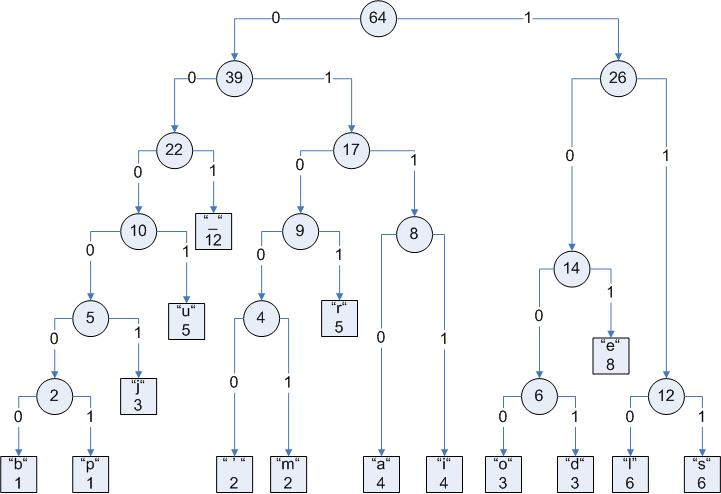
\includegraphics[scale=0.6]{fig/sunario-3/Huffman.jpg}%
	\caption{Hasil pohon }%
	\label{fig:Huffman Tree}%
\end{center}
\end{figure}

Pohon Huffman berfungsi pada proses Encoding dan Decoding data dengan syarat bahwa encoder dan decoder sudah sepakat untuk menggunakan Huffman tree tertentu sebelum terjadi pengiriman data. Encoder membangun Huffman tree yang baru setiap data baru akan dikirimkan, dan mengirimkan tabel konversi bersama-sama dengan data.

Untuk Algoritma Huffman mempunyai kompleksitas $O(n log n)$ untuk himpunan dengan n karakter.	

\section{\textit{Knapsack Problem}}

\textit{Knapsack Problem} merupakan suatu permasalahan bagaimana memilih objek dari sekian banyak dan  berapa besar objek tersebut akan disimpan sehingga diperoleh suatu penyimpanan yang optimal dengan memperhatikan objek yang terdiri dari n objek (1,2,3,...) dimana setiap objek memiliki  bobot (Wi) dan profit (Pi) dengan memperhatikan juga kapasitas dari media penyimpanan sebesar M dan nilai probabilitas dari setiap objek (Xi). Contoh permasalahan ini dalam dunia nyata adalah pedagang keliling dengan menggunakan gerobak ataupun alat pengangkut lainnya yang hanya memiliki kapasitas angkut maksimum sebesar w kg barang yang akan dijual.Barang yang dijual berjumlah satu untuk tiap jenisnya dan tiap jenis barang memiliki berat w1,w2,w3,w4, ..wn dengan keuntungan yang diperoleh untuk tiap jenisnya adalah p1,p2,p3,p4, .pn. Tetapi tidak semua jenis barang yang akan dijual oleh pedagang keliling tersebut dapat dimasukan kedalam alat pengangkut. Maka akan dipilih jenis-jenis barang yang akan dijual untuk setiap harinya oleh pedagang keliling tersebut agar diperoleh keuntungan yang maksimal dari penjualan barang-barang  tersebut. 

\subsection{Knapsack $0/1$}
knapsack 0/1, merupakan suatu masalah untuk memilih objek diambil, dengan ketentuan objek yang diambil harus seluruh diambil atau tidak sama sekali. Setiap   objek  tersebut mempunyai   nilai   keuntungan   atau   yang   disebut   dengan   profit.	Tujuan dari profit tersebut adalah untuk mendapatkan profit   yang   maksimal. Untuk   mendapatkan profit maksimal, tidak dapat ditentukan dari  banyak   objek   yang   masuk. Bisa saja hal yang sebaliknya yang terjadi. 

\begin{table}[h]
\begin{center}
\begin{tabular}{|c|c|c|c|}
\hline
W1 & 3  & p1 & 12 \\
W2 & 6  & p2 & 18\\
W3 & 5  & p3 & 10\\
W4 & 10  & p4 & 50\\
\hline
\multicolumn{4}{ |c| }{W maksimal = 16}\\
\hline
\end{tabular}
\caption{Data Masukkan}
\end{center}
\end{table}

Pada algoritma Greedy ada beberapa strategi yang digunakan untuk memilih objek yang akan dimasukkan kedalam knapsack seperti table 1.1 diatas, yaitu:
\begin{enumerate}
\item Greedy by profit \newline
Pada setiap langkah, knapsack diisi dengan objek yang mempunyai keuntungan terbesar. Strategi ini mencoba memaksimumkan keuntungan dengan memilih objek yang paling menguntungkan terlebih dahulu.

Pertama kali dilakukan adalah menurutkan secara menurun obyek-obyek berdasarkan profitnya .  Kemudian obyek-obyek yang dapat ditampung oleh knapsack diambil satu persatu sampai knapsack penuh atau (sudah tidak ada obyek lagi yang bisa dimasukan).
\begin{table}[h]
\begin{center}
\begin{tabular}{|c|c|c|c|c|}
\hline
\multicolumn{5}{ |c| }{Objek}\\
\hline
i & wi  & pi & pi/wi & status \\
\hline
4 & 10  & 50 & 5 & 1 \\
2 & 6  & 18 & 3 & 1 \\
3 & 5  & 10 & 2 & 0 \\
1 & 3  & 12 & 4 & 0 \\
\hline
\end{tabular}
\caption{Greedy by profit}
\end{center}
\end{table}
\item Greedy by weight.\newline
Pada setiap langkah, knapsack diisi dengan objek yang mempunyai berat paling ringan. Strategi ini mencoba memaksimumkan keuntungan dengan memasukkan sebanyak mungkin objek ke dalam knapsack.

Pertama kali yang dilakukan adalah mengurutkan secara menaik objek-objek berdasarkan weight-nya. Kemudian obyek-obyek yang dapat ditampung oleh knapsack diambil satu persatu sampai knapsack penuh atau (sudah tidak ada obyek lagi yang bisa dimasukan).
\begin{table}[h]
\begin{center}
\begin{tabular}{|c|c|c|c|c|}
\hline
\multicolumn{5}{ |c| }{Objek}\\
\hline
i & wi  & pi & pi/wi & status \\
\hline
1 & 3  & 12 & 4 & 1 \\
3 & 5  & 10 & 2 & 1 \\
2 & 6  & 18 & 3 & 1 \\
4 & 10  & 50 & 5 & 0 \\
\hline
\end{tabular}
\caption{Greedy by weight}
\end{center}
\end{table}
\item   Greedy by density. \newline
Pada setiap langkah, knapsack diisi dengan objek yang mempunyai densitas,  $pi / wi$ terbesar. Strategi ini mencoba memaksimumkan keuntungan dengan memilih objek yang mempunyai keuntungan per unit berat terbesar.

Pertama kali yang dilakukan adalah mencari nilai profit per unit/ density dari tiap-tiap objek. Kemudian obyek-obyek diurutkan berdasarkan densitasnya.
Kemudian obyek-obyek yang dapat ditampung oleh knapsack diambil satu persatu sampai knapsack penuh atau (sudah tidak ada obyek lagi yang bisa dimasukan).

\begin{table}[h]
\begin{center}
\begin{tabular}{|c|c|c|c|c|}
\hline
\multicolumn{5}{ |c| }{Objek}\\
\hline
i & wi  & pi & pi/wi & status \\
\hline
4 & 10  & 50 & 5 & 1 \\
1 & 3  & 12 & 4 & 1 \\
2 & 6  & 18 & 3 & 0 \\
3 & 5  & 10 & 2 & 0 \\
\hline
\end{tabular}
\caption{Greedy by weight}
\end{center}
\end{table}
\end{enumerate}

Perbandingan hasil optimal Penggunaan 3 strategi diatas Hal dapat dilihat pada tabel 1.5 berikut ini:

\begin{table}[h]
\begin{center}
\begin{tabular}{|c|c|c|c|c|c|c|c|}
\hline
\multicolumn{4}{ |c| }{Objek} & \multicolumn{3}{|c|}{Greddy by}  & \multirow{2}{*}{Solusi Optimal} \\
\hline 
i & wi  & pi & pi/wi & profit & weight & density \\
\hline
1 & 3  & 12 & 4 & 0 & 1 & 1 & 0\\
2 & 6  & 18 & 3 & 1 & 1 & 0 & 1\\
3 & 5  & 10 & 2 & 0 & 1 & 0 & 0\\
4 & 10  & 50 & 5 &1 & 0 & 1 & 1\\
\hline
\multicolumn{4}{ |r| }{Total Bobot} &16 & 14 & 13 & 16\\
\hline
\multicolumn{4}{ |r| }{Total Keuntungan} &68 & 40 & 62 & 68\\
\hline
\end{tabular}
\caption{}
\end{center}
\end{table}

Algoritma \textit{knapsack 0/1} dalam bahasa phyton dapat dituliskan sebagai berikut :

\lstset{language=Python}
\label{lst:Knapsack 0/1}
\begin{lstlisting}[frame=single]
def knapsack(v,w,n,W):
 V = [[for x in range(W+1)] for x in range(len(v)+1)]
 for j in range(W+1):
  V[0][j] = 0
	
 for i in range(1,n+1):
  for wx in range(W+1):
   if w[i-1] <= wx:
    V[i][wx] = max(V[i-1][wx], v[i-1]+V[i-1][wx-w[i-1]])
   else:
    V[i][wx] = V[i-1][wx]
		
 return V[n][W] 
\end{lstlisting}

Kompleksitas waktu algoritma di atas (dengan mangabaikan waktu pengurutan objek) adalah O(nW). 

\subsection{Fractional Knapsack}

Berbeda dengan knapsack 0/1, Fractional Knapsack merupakan suatu masalah untuk memilih objek diambil, dengan ketentuan objek hanya dapat diambil sebagian. Algoritma Greedy dalam hal ini memperoleh solusi dari masalah dengan membuat urutan pilihan. Ide dasarnya adalah untuk menghitung  rasio untuk setiap objek berdasarkan   bobot (Wi)  / profit (Pi) (Wi/Pi), dan diurutkan sesuai dengan rasionya. Kemudian objek dengan rasio tertinggi ditambahkan sampai objek tidak dapat diambil lagi. 

Sebagai contoh:\newline

\begin{table}[h]
\begin{center}
\begin{tabular}{|c|c|c|c|}
\hline
w1 & 18&    p1 & 25 \\
w2 & 15&    p2 & 24 \\
w3 & 10&    p3 & 15 \\
\hline
\multicolumn{4}{ |c| }{W maksimal = 20}\\
\hline
\end{tabular}
\caption{Data Masukkan}
\end{center}
\end{table}

Solusi dengan algoritma greedy dalam penyelesaian persoalan knapsack yang memakai strategi pemilihan objek berdasarkan pi /wi terbesar memberikan keuntungan yang maksimum (optimum). Agar proses pemilihan objek berikutnya optimal, maka kita perlu mengurutkan objek terlebih dahulu berdasarkan pi /wi dalam urutan yang menurun,  sehingga objek berikutnya yang dipilih adalah objek sesuai dalam urutan

\begin{table}[h]
\begin{center}
\begin{tabular}{|c|c|c|c|c|c|c|}
\hline
\multicolumn{4}{ |c| }{Objek} & \multicolumn{3}{|c|}{Greddy by}  \\
\hline 
i & wi  & pi & pi/wi & profit & weight & density \\
\hline
2 & 15 & 24 & 1,6 & $2/15$ & $2/3$ & 1\\
3 & 10 & 15 & 1,5 & 0 & 1 & $1/2$ \\
1 & 18 & 25 & 1,4 & 1 & 0 & 0 \\

\hline
\multicolumn{4}{ |r| }{Total Bobot} &20 & 20 & 20 \\
\hline
\multicolumn{4}{ |r| }{Total Keuntungan} &28,2 & 31,0 & 31,5 \\
\hline
\end{tabular}
\caption{Tabel Hasil Fractional Knapsack}
\end{center}
\end{table}

Solusi optmal persoalan knapsack di atas adalah X = (0, 1, 1/2) yang dimana dapat memberikan keuntungan maksimum 31,5.

Algoritma \textit{Fractional Knapsack} dalam bahasa phyton dapat dituliskan sebagai berikut :

\lstset{language=Python}
\label{lst:Fractional Knapsack}
\begin{lstlisting}[frame=single]
def knapsack(v,w,W):
 x=[]
 weight = 0
 i=0;
 while(weight<W):
  if(weight+w[i]<=w):
	 x[i]=1;
	 weight = weight +w[i]
	else:
	 x[i] = (w-weight)/w[i]
	 weight = W
 i+=1;
return x 
\end{lstlisting}

Kompleksitas waktu algoritma di atas (dengan mangabaikan waktu pengurutan objek) adalah O(n). 

\section{\textit{Algoritma Dijkstra}}
Salah satu permasalahan yang berkaitan dengan optimisasi adalah menentukan lintasan terpendek dari suatu tempat ke tempat yang lain.Permasalahan ini dapat diselesaikan dengan sebuah metode yang menggunakan perhitungan matematika eksak yaitu Algoritma Dijkstra.

Algoritma Dijkstra adalah algoritma dijkstra beroperasi secara menyeluruh terhadap semua alternatif fungsi yang ada sehingga rute terpendek yang didapat hanya dari titik awal sampai titik tujuan. Algoritma ini menggunakan prinsip greedy. Prinsip greedy pada algoritma dijkstra menyatakan bahwa pada setiap langkah,  pilih sisi yang berbobot minimum dan memasukannya dalam himpunan solusi. Cara kerja dari algoritma dijkstra adalah sebagai berikut:
\begin{enumerate}
\item Pada awalnya pilih sisi dengan bobot terendah dari node yang belum terpilih, diinisialisasi dengan 0 dan yang sudah terpilih diinisialisasi dengan 1.
\item Bentuk tabel yang terdiri dari titik ,status, bobot dan predecessor. Lengkapi kolom bobot yang diperoleh dari jarak titik sumber ke semua titik yang terhubung langsung dengan titik sumber tersebut
\item Jika titik sumber telah ditemukan maka tetapkanlah titik tersebut sebagai titik pilihan.
\item Tetapkan titik terpilih dengan label permanen dan perbaharui titik yang langsung terhubung.
\item Kemudian proses kembali titik sementara yang terhubung pada titik terpilih yang sudah diproses sebelumnya, dan merupakan titik dengan bobot terkecil dilihat dari tabel dan tentukan sebagai titik terpilih berikutnya.
\item Apakah titik terpilih merupakan titik tujuan? Jika ya, maka kumpulan titik terpilih atau predecessor merupakan rangkaian yang menunjukan lintasan terpendek .
\item Begitu seterusnya hingga semua titik sementara tersebut diubah statusnya menjadi titik terpilih.

Adapun lintasan terpendek dari Figur~\ref{fig:Jalur terpendek} yang akan diselesaikan dengan algoritma dijkstra dimana verteks awal adalah node A dan verteks tujuan adalah node J :

\begin{figure}[htbp]
\begin{center}
	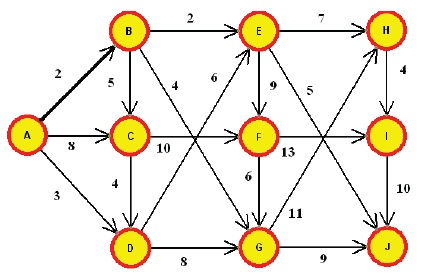
\includegraphics[scale=0.8]{fig/sunario-3/Graf.jpg}%
	\caption{Graf untuk Algoritma Dijkstra}%
	\label{fig:Jalur terpendek}%
\end{center}
\end{figure}

Penyelesaian Figur~\ref{fig:Jalur terpendek} dengan Algoritma Dijkstra ini adalah:
Tentukan bobot dari node yang langsung terhubung dengan node sumber yaitu node A, seperti dari node A ke node B = 2, A ke C = 8, dari A ke D = 3, dan untuk node E,F,G,H,I,J diinisialisasi dengan tanda „-„ karena tidak ada lintasan yang menghubungkan secara langsung dengan node A. kemudian predecessor(node sumber) dari A,B,C,D adalah A, karena jarak dari node tersebut dihitung dari node A, untuk node F,G,H,I,J predecessornya diberi tanda „-„ karena belum ada predecessor yang terhubung langsung dengan node tersebut.

\begin{table}[htbp]
\begin{center}
\begin{tabular}{|c|c|c|c|c|c|c|c|c|c|c|}
\hline
Node & A & B & C & D & E & F & G & H & I & J \\
\hline
Status & 1 & 0 & 0 & 0 & 0 & 0 & 0 & 0 & 0 & 0\\
\hline
Bobot & - & 2 & 8 & 3 & - & - & - & - & - & - \\
\hline
Predecessor & A & A & A & A & - & - & - & - & -  & - \\
\hline
\end{tabular}
\caption{Hasil Iterasi ke-1}
\end{center}
\end{table}

Dari hasil iterasi tabel 1.6 pilih node dengan status „0‟ dan bobot yang paling kecil yaitu B.untuk itu status node B menjadi „1‟ dan predecessornya tetap masih A. jika node B sudah terpilih, maka ada perubahan pada bobot node C,yaitu dari bobot 8 menjadi bobot 7,hal ini terjadi karena bobot 8 didapat dari node A langsung ke node C, padahal ada jalur yang lebih pendek untuk mencapai node C yaitu melewati B, dengan bobot 7, sehingga predecessor pada node C diganti menjadi B, dan karena node B sudah terpilih maka diperoleh node E dengan bobot 4(2+2) dan node G dengan bobot 6(2+4),predecessor node E dan G adalah B. Sehingga diperoleh :

\begin{table}[htbp]
\begin{center}
\begin{tabular}{|c|c|c|c|c|c|c|c|c|c|c|}
\hline
Node & A & B & C & D & E & F & G & H & I & J \\
\hline
Status & 1 & 1 & 0 & 0 & 0 & 0 & 0 & 0 & 0 & 0\\
\hline
Bobot & - & 2 & 7 & 3 & 4 & - & 6 & - & - & - \\
\hline
Predecessor & A & A & B & A & B & - & B & - & -  & - \\
\hline
\end{tabular}
\caption{Hasil Iterasi ke-2}
\end{center}
\end{table}

dapat dilihat dari tabel 1.7 bahwa node D merupakan node dengan bobot paling kecil dibandingkan dengan node-noode sementara yang ada, sehingga status node D sekarang akan berubah menjadi „1‟ dan predecessornya masih tetap A karena jalur terpendek menuju D adalah dari node A. sehingga diperoleh :

\begin{table}[htbp]
\begin{center}
\begin{tabular}{|c|c|c|c|c|c|c|c|c|c|c|}
\hline
Node & A & B & C & D & E & F & G & H & I & J \\
\hline
Status & 1 & 1 & 0 & 1 & 0 & 0 & 0 & 0 & 0 & 0\\
\hline
Bobot & - & 2 & 7 & 3 & 4 & - & 6 & - & - & - \\
\hline
Predecessor & A & A & B & A & B & - & B & - & -  & - \\
\hline
\end{tabular}
\caption{Hasil Iterasi ke-3}
\end{center}
\end{table}

Dari tabel 1.8 selanjutnya didapat bahwa node E memiliki bobot paling kecil, sehingga statusnya berubah menajadi „1‟. Jika node E sudah terpilih, maka node F mempunyai bobot 13, node H=11 dan node j=9 .untuk mencapai node F,H dan J maka harus dari node A kemudian ke node B lalu menuju node E maka predecessor ketiga node tersebut menjadi E. Sehingga diperoleh:

\begin{table}[htbp]
\begin{center}
\begin{tabular}{|c|c|c|c|c|c|c|c|c|c|c|}
\hline
Node & A & B & C & D & E & F & G & H & I & J \\
\hline
Status & 1 & 1 & 0 & 1 & 1 & 0 & 0 & 0 & 0 & 0\\
\hline
Bobot & - & 2 & 7 & 3 & 4 & 13 & 6 & 11 & - & 9 \\
\hline
Predecessor & A & A & B & A & B & E & B & E & -  & E \\
\hline
\end{tabular}
\caption{Hasil Iterasi ke-4}
\end{center}
\end{table}

Kemudian dari tabel 1.9 didapat bahwa node G memiliki bobt paling kecil, sehingga statusnya akan berubah menjadi „1‟, predecessornya masih tetap B. jika node G sudah terpilih maka akan ada perubahan bobot pada node F dari bobot 13 menjadi 12, hal ini terjadi karena setelah dihitung rute terpendek menuju F adalah dari node G kalau dibandingkan dengan rute dari node E maka predecessor node F berubah dari E menjadi G. sehingga diperoleh :

\begin{table}[htbp]
\begin{center}
\begin{tabular}{|c|c|c|c|c|c|c|c|c|c|c|}
\hline
Node & A & B & C & D & E & F & G & H & I & J \\
\hline
Status & 1 & 1 & 0 & 1 & 1 & 0 & 1 & 0 & 0 & 0\\
\hline
Bobot & - & 2 & 7 & 3 & 4 & 12 & 6 & 11 & - & 9 \\
\hline
Predecessor & A & A & B & A & B & G & B & E & -  & E \\
\hline
\end{tabular}
\caption{Hasil Iterasi ke-5}
\end{center}
\end{table}

Dan seterusnya algoritma ini akan terus mengulang semua proses yang ada hingga seluruh node yang berstatus sementara „0‟ diubah menjadi berstatus terpilih „1‟, hal ini dapat dilihat dari tabel dan gambar dibawah ini sampai iterasi ke-10:

\begin{table}[htbp]
\begin{center}
\begin{tabular}{|c|c|c|c|c|c|c|c|c|c|c|}
\hline
Node & A & B & C & D & E & F & G & H & I & J \\
\hline
Status & 1 & 1 & 1 & 1 & 1 & 0 & 1 & 0 & 0 & 0\\
\hline
Bobot & - & 2 & 7 & 3 & 4 & 12 & 6 & 11 & - & 9 \\
\hline
Predecessor & A & A & B & A & B & G & B & E & -  & E \\
\hline
\end{tabular}
\caption{Hasil Iterasi ke-6}
\end{center}
\end{table}

\begin{table}[htbp]
\begin{center}
\begin{tabular}{|c|c|c|c|c|c|c|c|c|c|c|}
\hline
Node & A & B & C & D & E & F & G & H & I & J \\
\hline
Status & 1 & 1 & 1 & 1 & 1 & 0 & 1 & 0 & 0 & 1\\
\hline
Bobot & - & 2 & 7 & 3 & 4 & 12 & 6 & 11 & 19 & 9 \\
\hline
Predecessor & A & A & B & A & B & G & B & E & J  & E \\
\hline
\end{tabular}
\caption{Hasil Iterasi ke-7}
\end{center}
\end{table}


\begin{table}[htbp]
\begin{center}
\begin{tabular}{|c|c|c|c|c|c|c|c|c|c|c|}
\hline
Node & A & B & C & D & E & F & G & H & I & J \\
\hline
Status & 1 & 1 & 0 & 1 & 1 & 0 & 1 & 1 & 0 & 0\\
\hline
Bobot & - & 2 & 7 & 3 & 4 & 12 & 6 & 11 & 15 & 9 \\
\hline
Predecessor & A & A & B & A & B & G & B & E & H  & E \\
\hline
\end{tabular}
\caption{Hasil Iterasi ke-8}
\end{center}
\end{table}

\begin{table}[htbp]
\begin{center}
\begin{tabular}{|c|c|c|c|c|c|c|c|c|c|c|}
\hline
Node & A & B & C & D & E & F & G & H & I & J \\
\hline
Status & 1 & 1 & 1 & 1 & 1 & 1 & 1 & 1 & 0 & 1\\
\hline
Bobot & - & 2 & 7 & 3 & 4 & 12 & 6 & 11 & 15 & 9 \\
\hline
Predecessor & A & A & B & A & B & G & B & E & H  & E \\
\hline
\end{tabular}
\caption{Hasil Iterasi ke-9}
\end{center}
\end{table}

\begin{table}[htbp]
\begin{center}
\begin{tabular}{|c|c|c|c|c|c|c|c|c|c|c|}
\hline
Node & A & B & C & D & E & F & G & H & I & J \\
\hline
Status & 1 & 1 & 1 & 1 & 1 & 1 & 1 & 1 & 1 & 1\\
\hline
Bobot & - & 2 & 7 & 3 & 4 & 12 & 6 & 11 & 15 & 9 \\
\hline
Predecessor & A & A & B & A & B & G & B & E & H  & E \\
\hline
\end{tabular}
\caption{Hasil Iterasi ke-10}
\end{center}
\end{table}

\newpage
\begin{figure}[htbp]
\begin{center}
	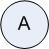
\includegraphics[scale=0.5]{fig/sunario-3/A.jpg}%
	\caption{Node Terpilih Hasil Iterasi 1}%
	\label{fig:Node A}%
\end{center}
\end{figure}


\begin{figure}[htbp]
\begin{center}
	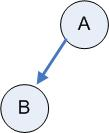
\includegraphics[scale=0.5]{fig/sunario-3/AB.jpg}%
	\caption{Node Terpilih Hasil Iterasi 2}%
\end{center}
\end{figure}


\begin{figure}[htbp]
\begin{center}
	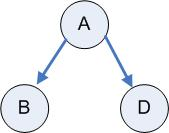
\includegraphics[scale=0.5]{fig/sunario-3/ABD.jpg}%
	\caption{Node Terpilih Hasil Iterasi 3}%
\end{center}
\end{figure}

\begin{figure}[htbp]
\begin{center}
	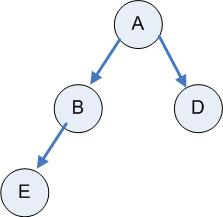
\includegraphics[scale=0.5]{fig/sunario-3/ABDE.jpg}%
	\caption{Node Terpilih Hasil Iterasi 4}%
\end{center}
\end{figure}


\begin{figure}[htbp]
\begin{center}
	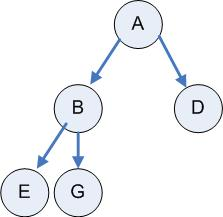
\includegraphics[scale=0.5]{fig/sunario-3/ABDEG.jpg}%
	\caption{Node Terpilih Hasil Iterasi 5}%
\end{center}
\end{figure}

\begin{figure}[htbp]
\begin{center}
	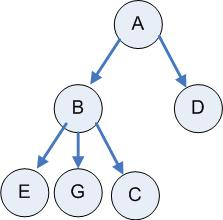
\includegraphics[scale=0.5]{fig/sunario-3/ABDEGC.jpg}%
	\caption{Node Terpilih Hasil Iterasi 6}%
\end{center}
\end{figure}

\begin{figure}[htbp]
\begin{center}
	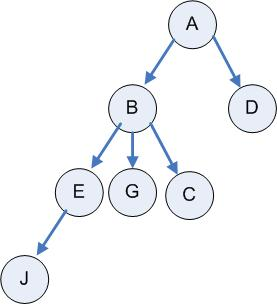
\includegraphics[scale=0.5]{fig/sunario-3/ABDEGCJ.jpg}%
	\caption{Node Terpilih Hasil Iterasi 7}%
\end{center}
\end{figure}

\begin{figure}[htbp]
\begin{center}
	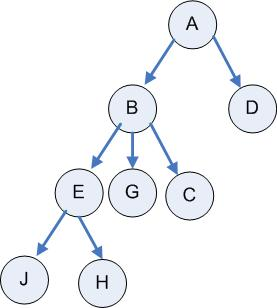
\includegraphics[scale=0.5]{fig/sunario-3/ABDEGCJH.jpg}%
	\caption{Node Terpilih Hasil Iterasi 8}%
\end{center}
\end{figure}


\begin{figure}[htbp]
\begin{center}
	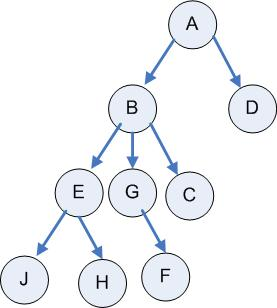
\includegraphics[scale=0.5]{fig/sunario-3/ABDEGCJHF.jpg}%
	\caption{Node Terpilih Hasil Iterasi 9}%
\end{center}
\end{figure}

\begin{figure}[htbp]
\begin{center}
	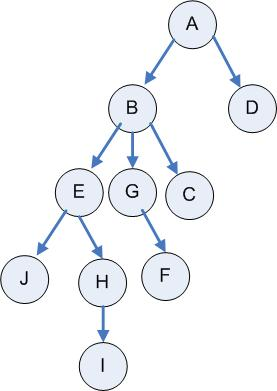
\includegraphics[scale=0.5]{fig/sunario-3/ABDEGCJHFI.jpg}%
	\caption{Node Terpilih Hasil Iterasi 10}%
\end{center}
\end{figure}

\newpage
Setelah mencapai iterasi ke-10 maka semua node yang ada telah berubah status menjadi node terpilih, sehingga akan terbentuk jalur terpendek dari node A ke semua node yang ada, untuk melihat jalur mana yang terpilih dapat ditelusuri dari predecessornya. Itulah yang membedakan algoritma dijkstra dengan algoritma heuristic dimana algoritma dijkstra tidak hanya mencari jalur terpendek dari node awal ke node tujuan tetapi kesemua node yang ada.hal ini dapat dilihat dibawah ini:

$A \triangleright B : A - B : 2 \newline$
$A \triangleright C : A - B - C : 7 \newline$
$A \triangleright D : A - D : 3 \newline$
$A \triangleright E : A - B - E : 4 \newline$
$A \triangleright F : A - B - G - F : 12 \newline$
$A \triangleright G : A - B - G : 6 \newline$
$A \triangleright H : A - B - E - H : 11 \newline$
$A \triangleright I : A - B - E - H - I : 15 \newline$
$A \triangleright J : A - B - E - J : 9 \newline$

Algoritma Dijistrak dalam bahasa phyton dapat dituliskan sebagai berikut :

\lstset{language=Python}
\label{lst:Djistrak}
\begin{lstlisting}[frame=single]
def Dijkstra(G,start,end=None):
 D = {}	# final distances
 P = {}	# predecessors
 Q = priorityDictionary()   #non-final vertex.
 Q[start] = 0
  for v in Q:
  D[v] = Q[v]
  if v == end: 
   break
  for w in G[v]:
  vwLength = D[v] + G[v][w]
  if w in D:
   if vwLength < D[w]:
  	raise ValueError, "Dijkstra: vertex final"   
   elif w not in Q or vwLength < Q[w]:
  	Q[w] = vwLength
  	P[w] = v
		
  return (D,P)
			
def shortestPath(G,start,end):
	D,P = Dijkstra(G,start,end)
	Path = []
	while 1:
		Path.append(end)
		if end == start: break
		end = P[end]
	Path.reverse()
	return Path
\end{lstlisting}

Untuk algoritma Dijkstra, kompleksitas waktu untuk
suatu graf dengan sisi E dan simpul V dapat diekspresikan
dalam bentuk suatu fungsi dari $|E|$ dan $|V|$ sebagai $O(|V^{2}| + |E|) = O(|V^{2}|)$. Dengan sedikit perbaikan, algoritma ini dapat mencapai $O(|E| + |V|) log| =
O(|E| log|V|) ≈ O(|E| + |V| log|V|)$.
\end{enumerate}
